\section{Ablations}
\label{sec:ablations_rewrite}

We carried out ablations on two tasks: finding tensor decompositions for faster matrix multiplication (\Cref{subsec:matmul}) and computing lower bounds on kissing numbers (\Cref{subsec:math}), aiming to understand the efficacy of the following components of \method.

\begin{itemize}
    \item {\bf Evolutionary approach.} \method utilizes an evolutionary approach, where previously generated programs are stored in a database and used to obtain better programs in subsequent iterations. To analyze the importance of evolution, we consider an alternative approach, which repeatedly feeds the same initial program to the language model. We refer to this approach as ``No evolution''.
    \item {\bf Context in prompts.} \method uses powerful language models with large context windows, whose output can be improved significantly by providing problem-specific context in the prompt. To test the importance of context, we consider an alternative approach where no explicit context is added to the prompt. We refer to this approach as ``No context in the prompt''.
    \item {\bf Meta prompts.} \method also uses meta prompts in order to improve the prompts that are provided to the language model. This allows it to potentially surpass the performance one can obtain using a human prompter. To test the efficacy of meta prompting, we disable it for the task of tensor decomposition. We refer to this approach as ``No meta prompt evolution''.
    \item {\bf Full-file evolution.} Unlike previous approaches such as FunSearch, \method can evolve an entire codebase instead of focusing on a single function. To test the importance of full-file evolution, we consider an alternative in the context of tensor decomposition where only the loss function is evolved. We refer to this approach as ``No full-file evolution''.
    \item {\bf Powerful language models.} \method relies on a mixture of small and large language models in order to obtain highly diverse samples. To understand the importance of this component, we consider an alternative where only a single small base model is used. We refer to this approach as ``Small base LLM only''.
\end{itemize}

\begin{figure}
\centering
\begin{subfigure}[c]{0.48\textwidth}
    \centering
    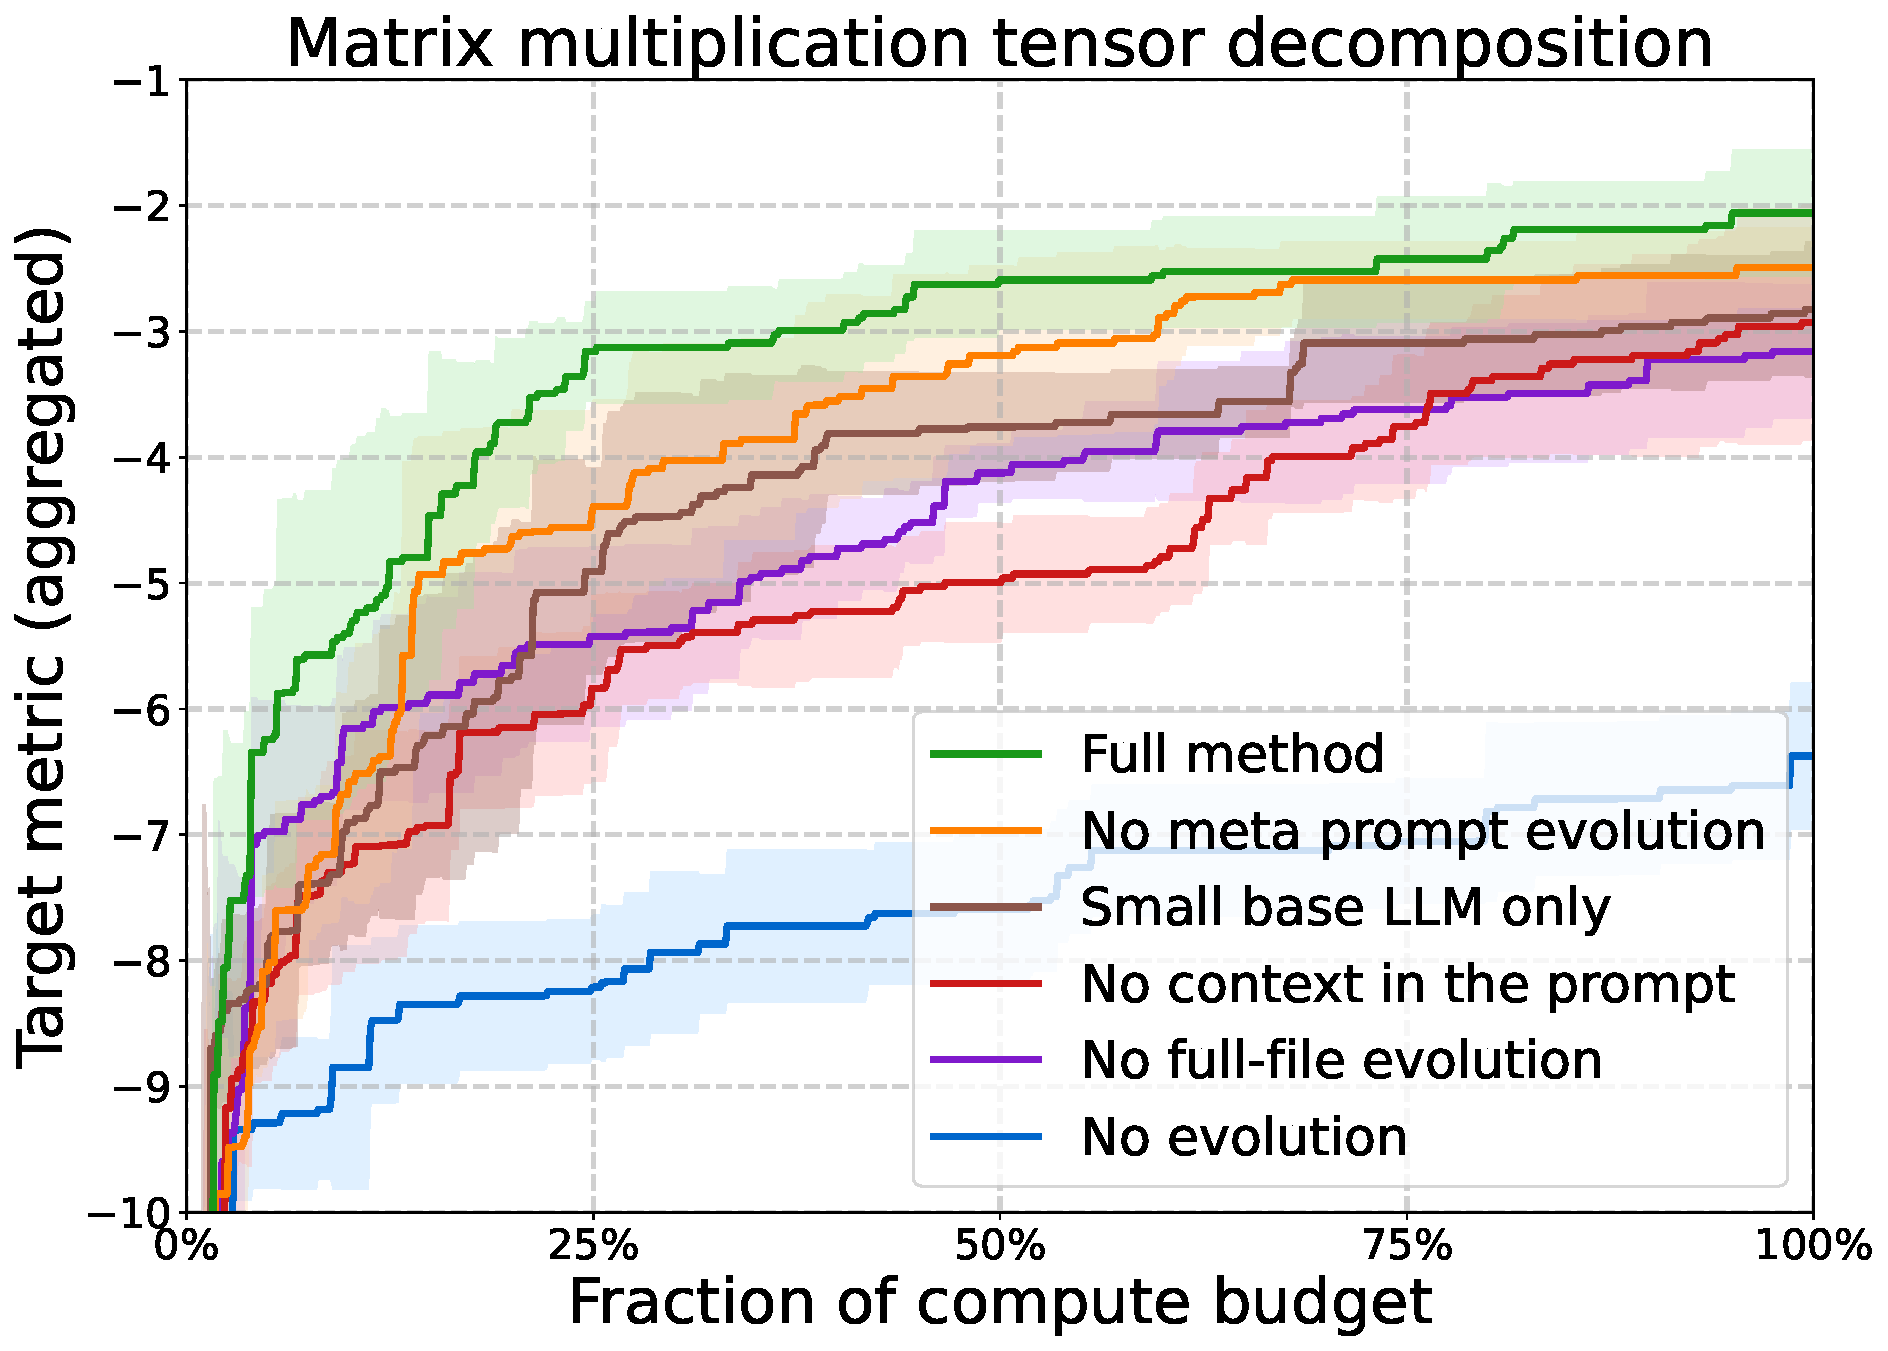
\includegraphics[width=1.0\textwidth]{figures/ablation_matmul.pdf}
\end{subfigure}%
\hfill
\begin{subfigure}[c]{0.48\textwidth}
    \centering
    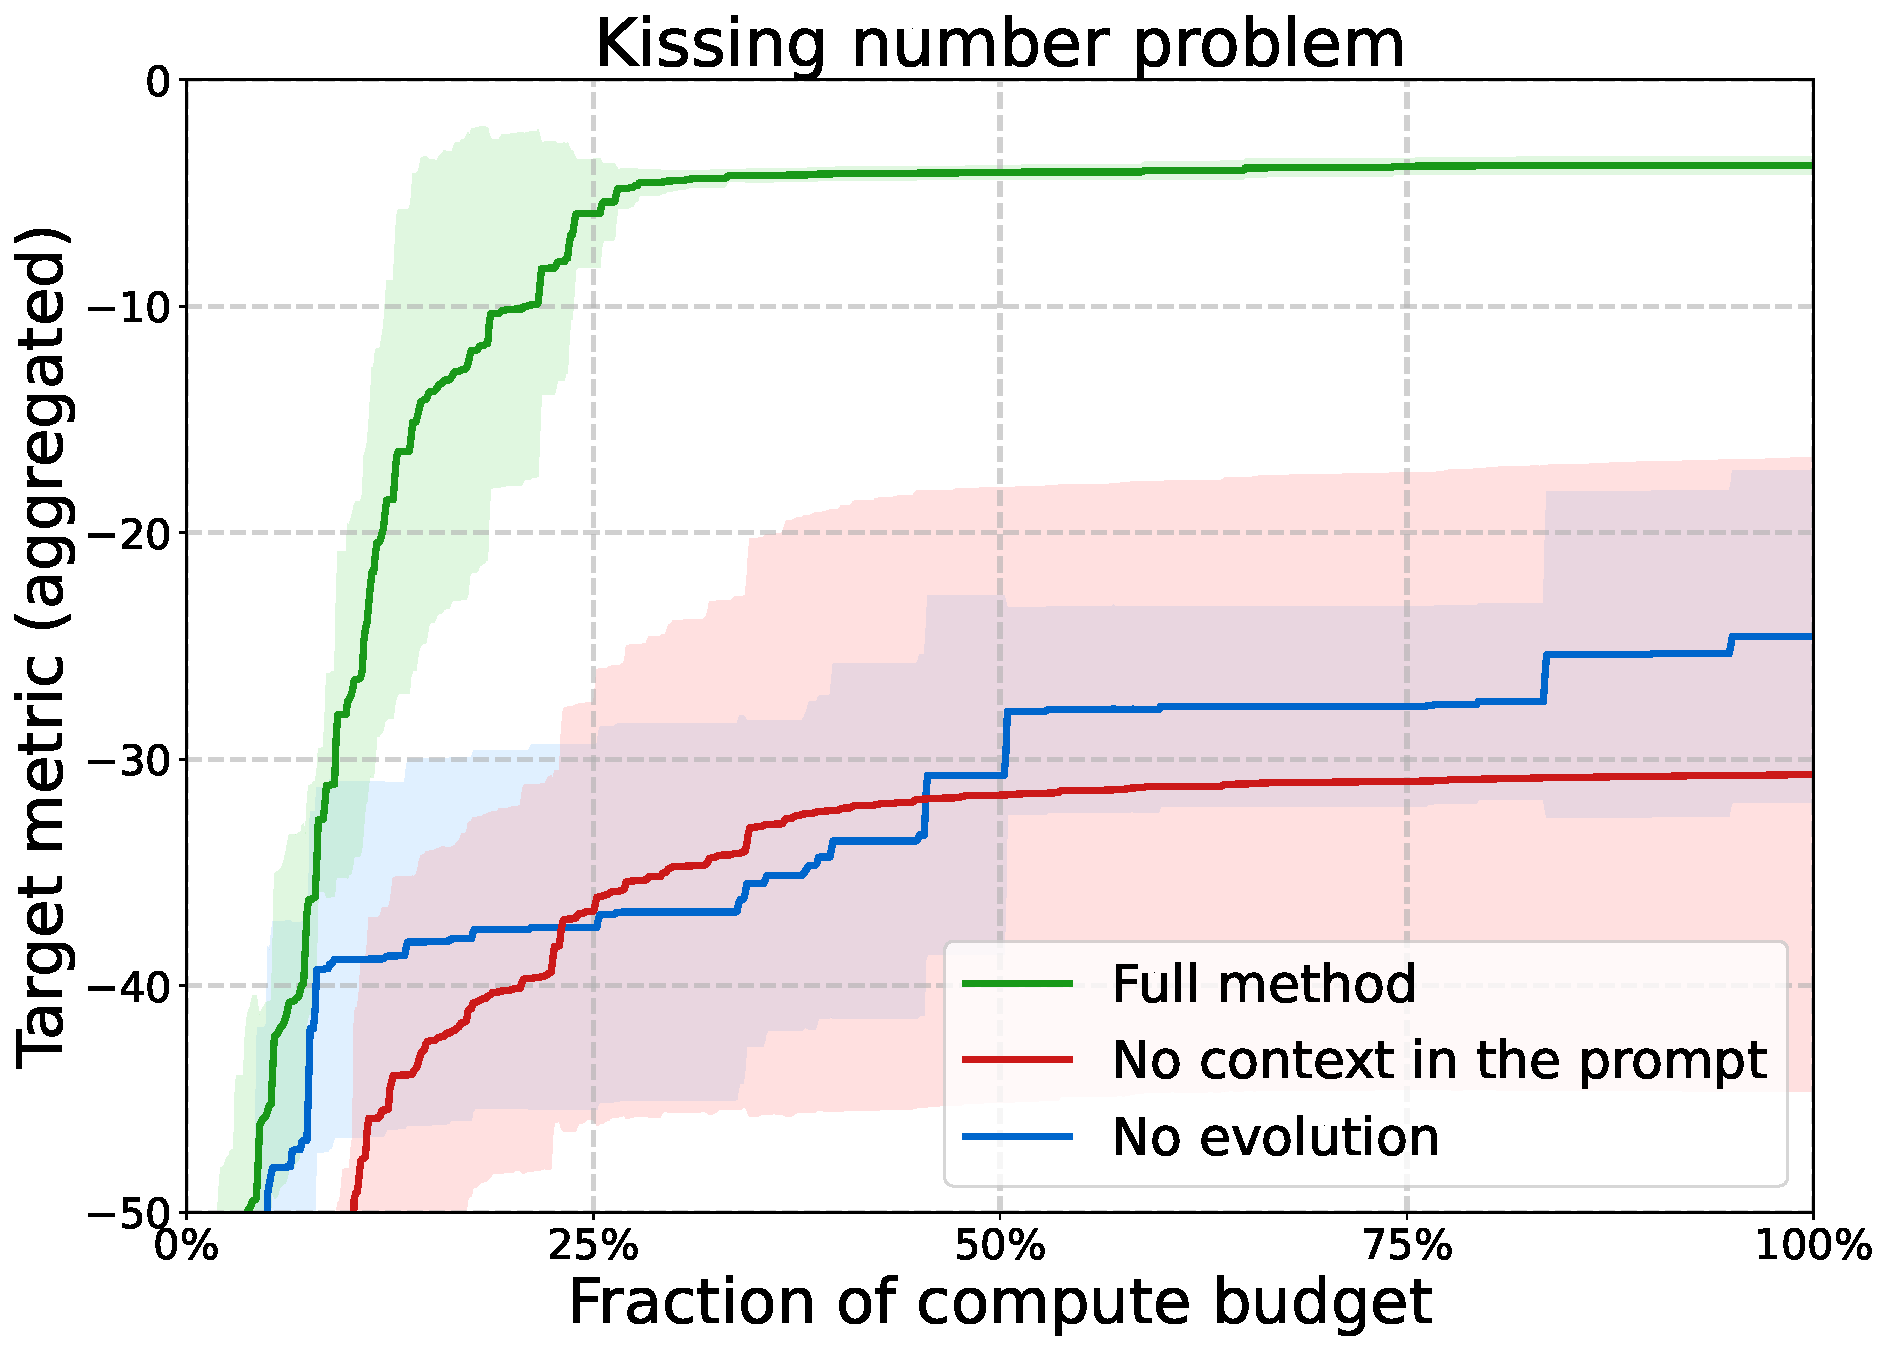
\includegraphics[width=1.0\textwidth]{figures/ablation_kissing.pdf}
\end{subfigure}%
\caption{Left: Ablations of \method on the problem of finding low-rank tensor decomposition for faster matrix multiplication. Right: Ablations of \method on the problem of finding sphere packings for improving kissing numbers. Each curve shows the performance of an individual setting with increasing compute budget, averaged over all considered targets (higher values on the target metric are better). The shades indicate intra-target standard deviation, averaged over three independent runs of \method, initialized with different random seeds.%
\label{fig:ablations_rewrite}}
\end{figure}

\Cref{fig:ablations_rewrite} shows the results of the all-inclusive \method approach as well as the various alternatives listed above. As can be seen, each of the components is responsible for a significant improvement in the results. 
